\documentclass[12pt]{article}
\title{ECE 141 Homework 4}
\usepackage{subcaption}
\author{Lawrence Liu}
\usepackage{graphicx}
\usepackage{amsmath}
\usepackage{placeins}
\newcommand{\Laplace}{\mathscr{L}}
\setlength{\parskip}{\baselineskip}%
\setlength{\parindent}{0pt}%
\usepackage{xcolor}
\usepackage{listings}
\definecolor{backcolour}{rgb}{0.95,0.95,0.92}
\usepackage{amssymb}
\lstdefinestyle{mystyle}{
    backgroundcolor=\color{backcolour}}
\lstset{style=mystyle}

\begin{document}
\maketitle
\section*{Problem 1}
We have that $$\beta=\arctan(\frac{l_r}{l_r+l_f}\tan(u))$$
therefore
$$\tan(\beta)=\frac{l_r}{l_r+l_f}\tan(u)$$
therefore since the range of $\tan$ is $-\infty$ to $\infty$ for any $\beta$ we can find a $u$ that satisfies the equation.

\section*{Problem 2}
We have that
$$\frac{d}{dt}y=v\sin(\psi+\beta)$$
$$\frac{d}{dt}\psi=\frac{v}{l_R}\sin(\beta)$$
$$\beta=\arctan(\frac{l_r}{l_r+l_f}\tan(u))$$
Linearizing around $\psi=0$ $\beta=0$, we have
$$\frac{d}{dt}y=v(\psi+\beta)$$
$$\frac{d}{dt}\psi=\frac{v}{l_R}\beta$$
therefore taking the laplace transform we have
$$sY=v(\psi+\beta)$$
$$s\psi=\frac{v}{l_r}\beta$$
Therefore we get
$$sY=v(\frac{v}{l_r s}+1)\beta$$
Therefore the transfer function is
$$\frac{Y(s)}{\beta}=\frac{v(v+l_r s)}{l_r s^2}$$
So now with a controller $D_c(s)$ and unity feedback we have that the transfer function is
$$\frac{Y}{R}=\frac{D_c(s)\frac{v(v+l_r s)}{l_r s^2}}{1+D_c(s)\frac{v(v+l_r s)}{l_r s^2}}$$

If the controller is a simple portional controller then the transfer function becomes
$$\frac{Y}{R}=\frac{k_pv(v+l_r s)}{l_r s^2+k_pv(v+l_r s)}$$
Therefore the transfer function for the error is 
$$\frac{E}{R}=1-\frac{k_pv(v+l_r s)}{l_r s^2+k_pv(v+l_r s)}$$
$$\frac{E}{R}=\frac{l_r s^2}{l_r s^2+k_pv(v+l_r s)}$$

Therefore for unit step input, which is what we will have, we have that the steady state error is 
$$\lim_{t\to\infty}e(\infty)=\lim_{s\to0}\frac{l_r s^2}{l_r s^2+k_pv(v+l_r s)}$$
$$\lim_{t\to\infty}e(\infty)=0$$
Therefore we must have characteristic polynomial
$$l_r s^2+k_pv(v+l_r s)=0$$
$$s^2+k_pvs+\frac{k_pv^2}{l_r}=0$$
In order for this system to be critically damped we must have that
$$2v\sqrt{\frac{k_p}{l_r}}=k_pv$$
therefore we have that $\sqrt{k_p}=\frac{2}{\sqrt{l_r}}$, and thus $k_p=\frac{4}{l_r}$. To confirm that this is indeed stable, and that the system is critically damped, we plot out
the poles and zeros of the system. Using the following matlab code, we get the pole zero plots
\begin{verbatim}
v=15.6464;
l_r=1.7;
k_p=4/l_r;

sys = tf([k_p*v*l_r k_p*v^2],[l_r  k_p*v*l_r k_p*v^2]);
h = pzplot(sys);
grid on
\end{verbatim}
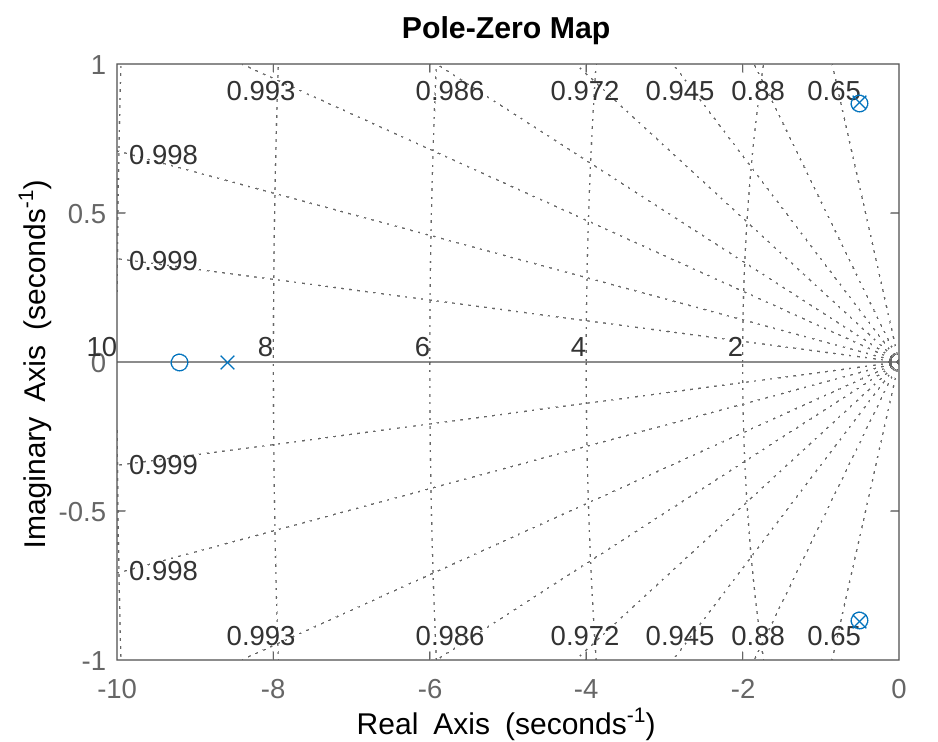
\includegraphics[scale=0.3]{Problem2Fig1.png}
As we can see, the system is critically damped since the poles are at the same place, furthermore the system is stable since the poles are all
less than 0.
\section*{Problem 3}
The blockdiagram for the nonlinear system looks like the following\\
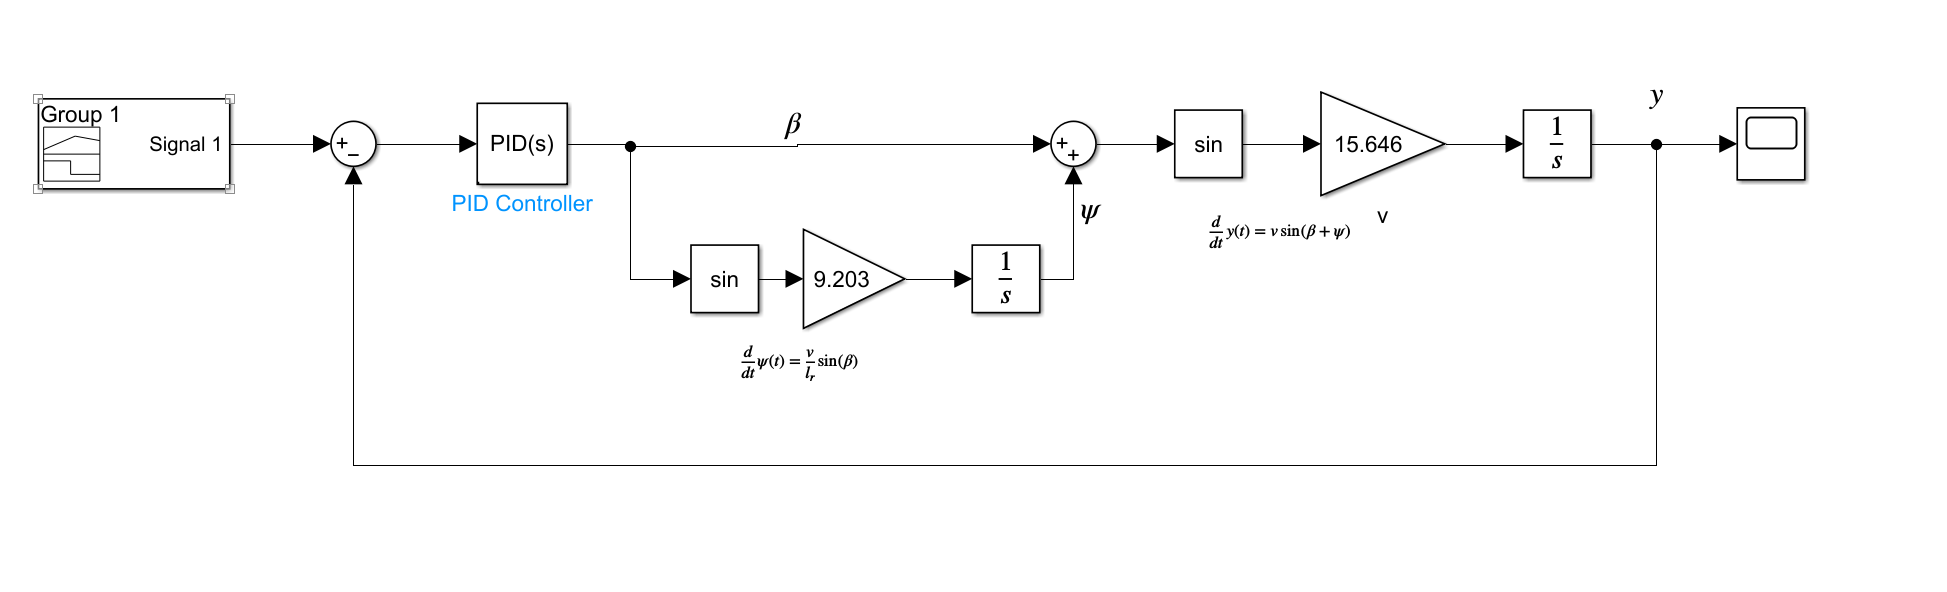
\includegraphics[scale=0.4]{Problem3BlockDiagram.PNG}\\
We can modify the initial conditions by modifying the inital conditions for the integrator blocks. We define acceptable behavior, 
as the car not oscillating, so the y value cannot exceed the initial y value, and cannot be less than 0 if we start the car with a positive y,
and vice versa for a negative initial y.
\\\\
Using the following matlab code we can plot out where the initial values of $y$ and $\psi$ result in acceptable behavior
\begin{verbatim}
l_r=1.7;
v=15.6464;
k_p=4/l_r;
psi_sweep=-pi/6:0.02:pi/6;
y_sweep=-2:0.05:-1;
t_final=40;
valid = zeros(length(psi_sweep),length(y_sweep));

for i=1:length(psi_sweep)
    psi_initial=psi_sweep(i);
    psi_initial
    for j=1:length(y_sweep)
        y_initial=10^(y_sweep(j));
        a=sim("Problem3.slx");

        data=a.yout.getElement("y");
        if max(abs(data.Values.Data))<=y_initial && min(data.Values.Data)>=0
            valid(i,j)=1;
        end
    end

end

imagesc(y_sweep,psi_sweep,valid)
colorbar
ylabel("\psi initial values")
xlabel("log(abs(y)) initial values")
\end{verbatim}
which outputs the following plot\\
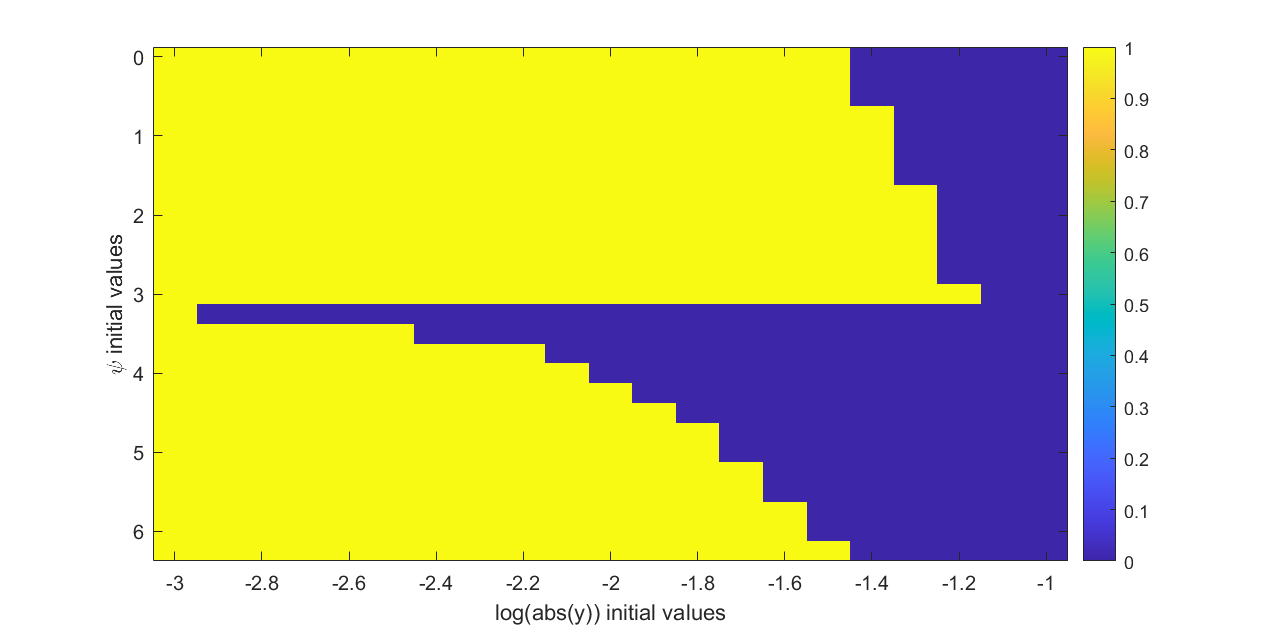
\includegraphics[scale=0.4]{Problem3Fig1.png}\\
Where the yellow block is the acceptable region, and the blue blocks are the unacceptable regions.\\
To check this, let us plot out the behavior of the system for the initial conditions $y(0)=0.1$ and $\psi(0)=0.1$\\
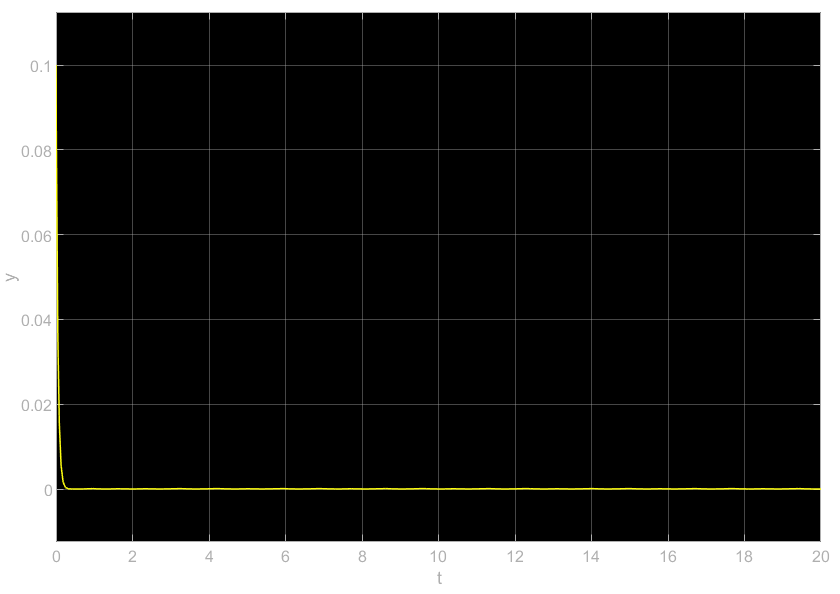
\includegraphics[scale=0.4]{Problem3Fig2.png}\\
As we can see, for these initial conditions, the system does not oscillate, so the performance is satisfactory. 
Now for the initial conditions $y(0)=0.1$ and $\psi(0)=\frac{\pi}{6}$, we get the following graph for y\\
\\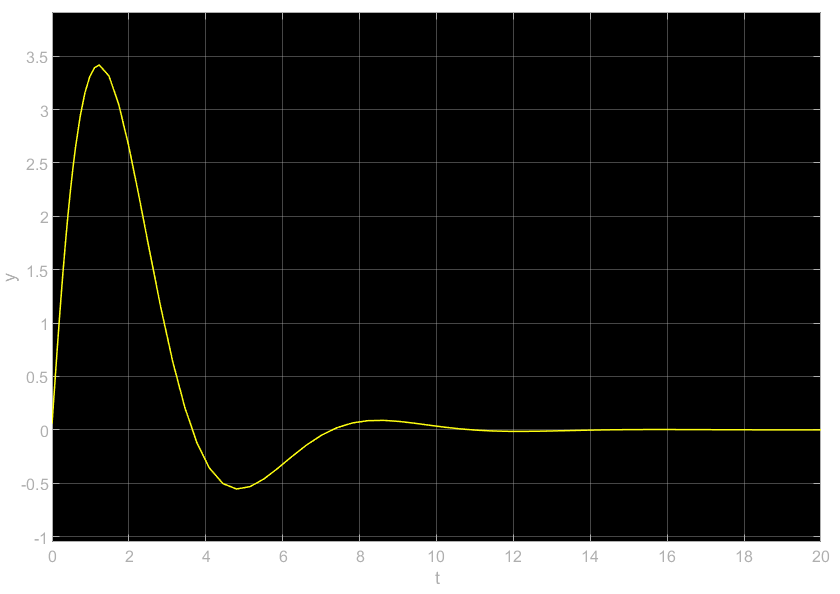
\includegraphics[scale=0.4]{Problem3Fig3.png}\\
As we can see for these initial conditions, the system oscillates, with y first increasing to more than $0.15$ before it decreases
So this performance is not satisfactory
\section*{Problem 4}
We have
$$\frac{d}{dt}v=a$$
$$sv=a$$
$$\frac{v}{a}=\frac{1}{s}$$
therefore with a pid controller the transfer function from the input target velocity to the output velocity is 
$$\frac{(k_p+k_ds+k_i\frac{1}{s})\frac{1}{s}}{1+(k_p+k_ds+k_i\frac{1}{s})\frac{1}{s}}$$
Therefore the characteristic polynomial is
$$s^2+(k_ps+k_ds^2+k_i)=0$$, Setting $k_d=0$ for now, we focus on making this system critically damped as well, since we would want
the car to match velocity as quickly as possible, but not for it to oscillate
then we have
$$s^2+k_ps+k_i=0$$
in order for this system to be critically damped, we want,
$$\sqrt{k_i}=\frac{k_p}{2}$$
We pick $k_p=1$ and $k_i=\frac{1}{4}$. To confirm we plot the poles and zeros of the system
\begin{verbatim}
k_p=1;
k_i=k_p^2/4;

sys = tf([k_p k_i],[1 k_p k_i]);
h = pzplot(sys);
grid on
\end{verbatim}
which outputs the following pole zero plot\\
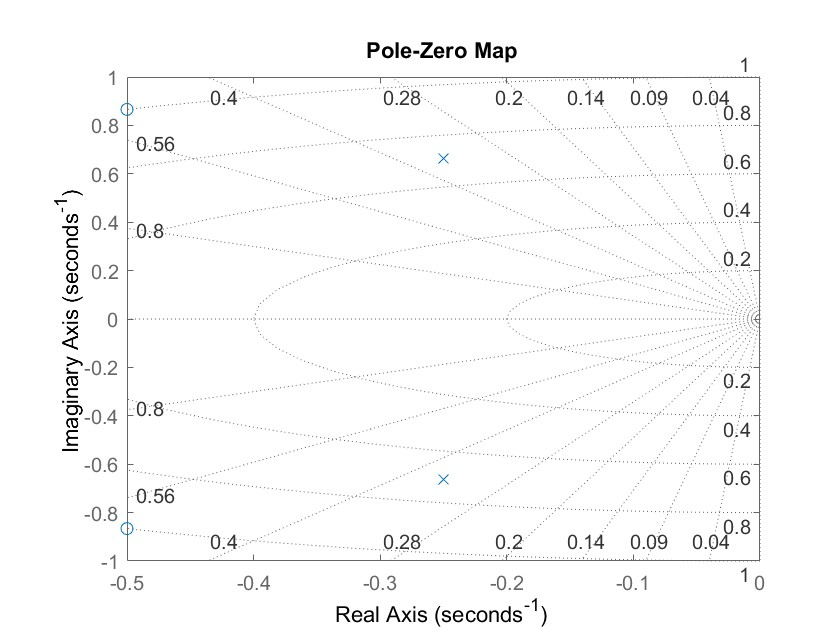
\includegraphics[scale=0.4]{Problem4Fig1.jpg}\\
As we can see, the system is critically damped since the poles are at the same place, furthermore the system is stable since the poles are all
less than 0.
\section*{Problem 5}
The blockdiagram for the nonlinear system looks like the following\\
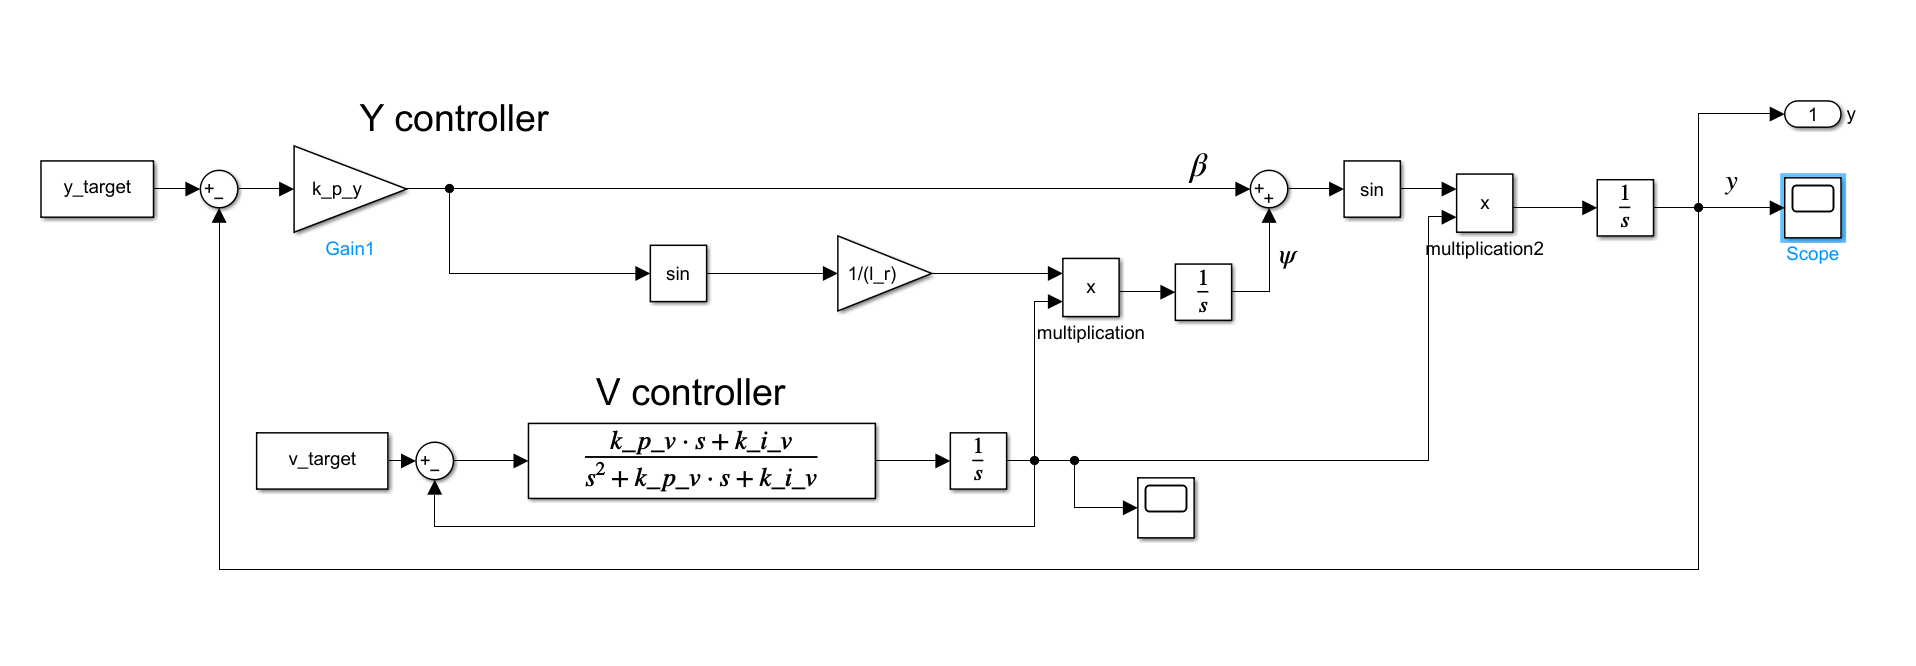
\includegraphics[scale=0.4]{Problem5BlockDiagram.PNG}\\
Using the following code we plot out the initial values of $y$ and $\psi$ result in acceptable behavior, when $v$ initially is $10m/s$, $15.6464m/s$, and $20m/s$.
We keep the same definition of acceptable behavior as before
\begin{verbatim}
    v_target=15.6464;
y_target=0;
l_r=1.7;

v_sweep=[10 15.6464 20];
log_y_sweep=-3:0.1:-1;
psi_sweep=0:0.25:2*pi;


for i=1:length(v_sweep)
v_initial=v_sweep(i)
f = figure;
valid = zeros(length(psi_sweep),length(log_y_sweep));
for j=1:length(psi_sweep)
    psi_initial=psi_sweep(j);
    for k=1:length(log_y_sweep)
        y_initial=10^(log_y_sweep(k));

        a=sim("Problem3.slx");

        data=a.yout.getElement("y");
    
        if max(abs(data.Values.Data))<0.6
            valid(j,k)=1;
        end
    end

end
imagesc(log_y_sweep,psi_sweep,valid);
colorbar
ylabel("\psi initial values")
xlabel("log(abs(y)) initial values")
title(['v= ',num2str(v_initial),' m/s'])
end
\end{verbatim}


which results in the following plots, for $v=20m/s$\\
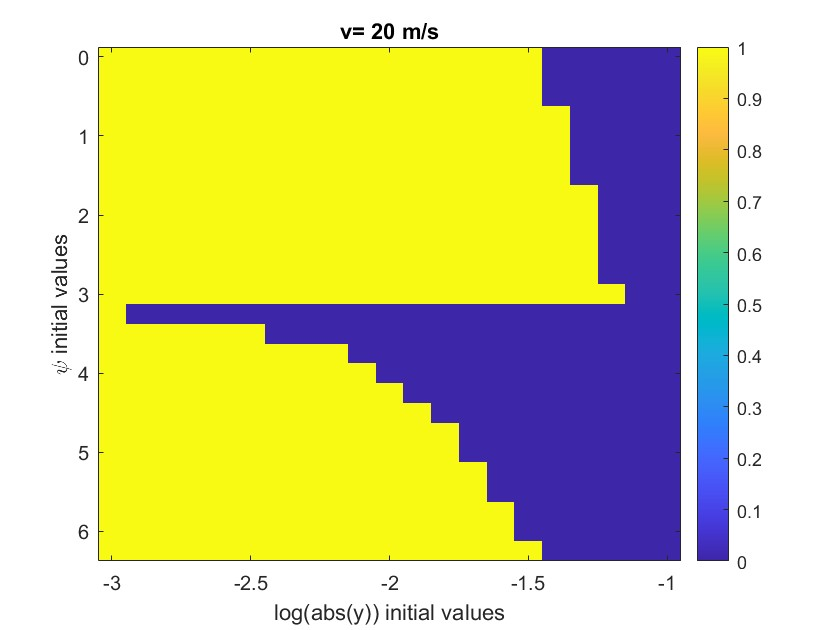
\includegraphics[scale=0.4]{Problem5v20.jpg}\\
for $v=15.6464m/s$\\
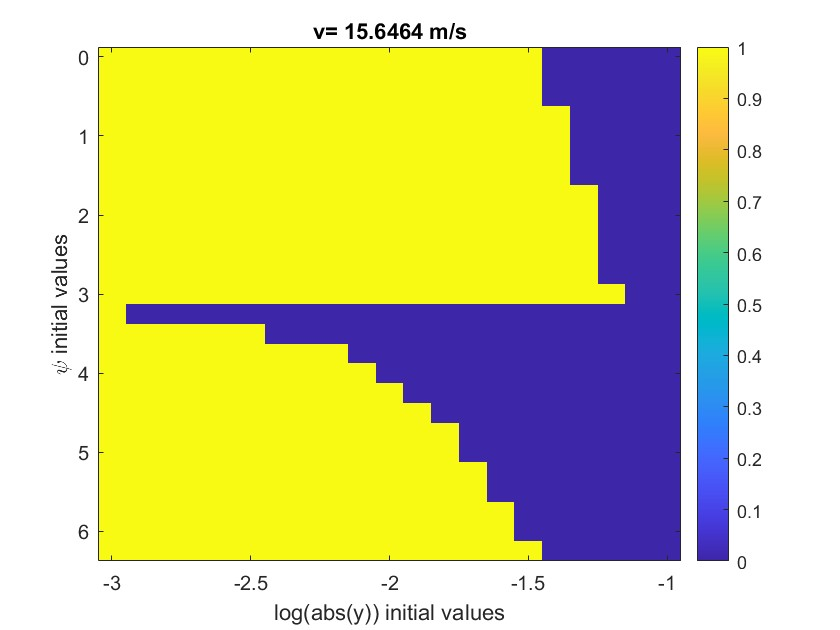
\includegraphics[scale=0.4]{Problem5v15.jpg}\\
and for $v=10m/s$\\
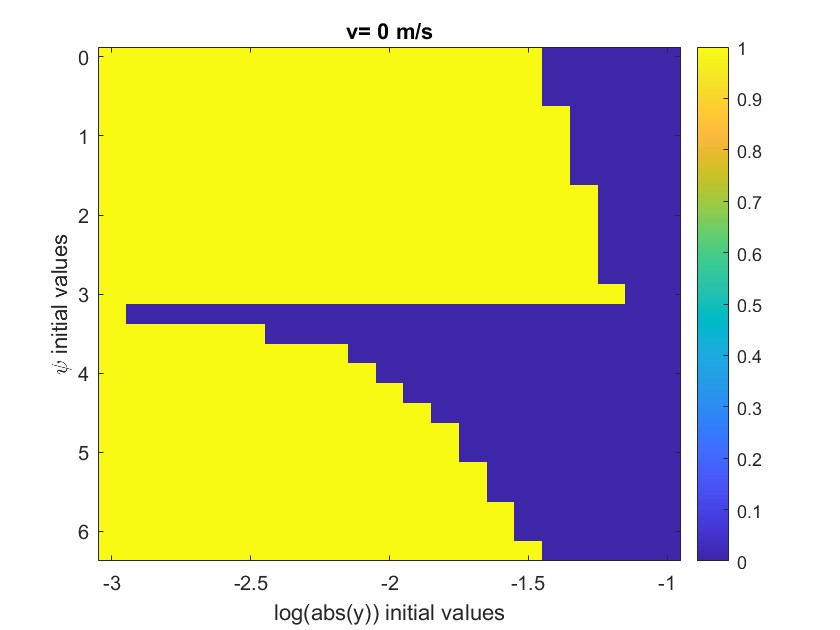
\includegraphics[scale=0.4]{Problem5v0.jpg}\\
As we can see changing the initial v does not seem to matter at all\\
To verify this we plot out the velocity and y for the initial conditions, $v(0)=0$, $y(0)=0.1$, $\psi(0)=0.1$,
 and for the initial conditions $v(0)=0$, $y(0)=0.1$, $\psi(0)=\frac{\pi}{6}=0.523$
Using the following code, we can do that
\begin{verbatim}
v_target=15.6464;
y_target=0;
l_r=1.7;


k_p_v=1;
k_i_v=k_p_v^2/4;
k_d_v=0;
k_p_y=4/l_r;
t_final=20;
max_step_size=0.0001;

y_initial=0.1;
psi_initial=0.1;
v_initial=0;

a=sim("Problem5.slx");
t=a.tout;
y=a.yout.getElement("y").Values.Data;
v=a.yout.getElement("v").Values.Data;

subplot(2,2,1); 
plot(t,y)
title(["y response for psi initial=",num2str(psi_initial)])

subplot(2,2,2); 
plot(t,v)
title(["v response for psi initial=",num2str(psi_initial)])

psi_initial=pi/6;
a=sim("Problem5.slx");
t=a.tout;
y=a.yout.getElement("y").Values.Data;
v=a.yout.getElement("v").Values.Data;

subplot(2,2,3); 
plot(t,y)
title(["y response for psi initial=",num2str(psi_initial)])

subplot(2,2,4); 
plot(t,v)
title(["v response for psi initial=",num2str(psi_initial)])
\end{verbatim}
We get the following graph.\\
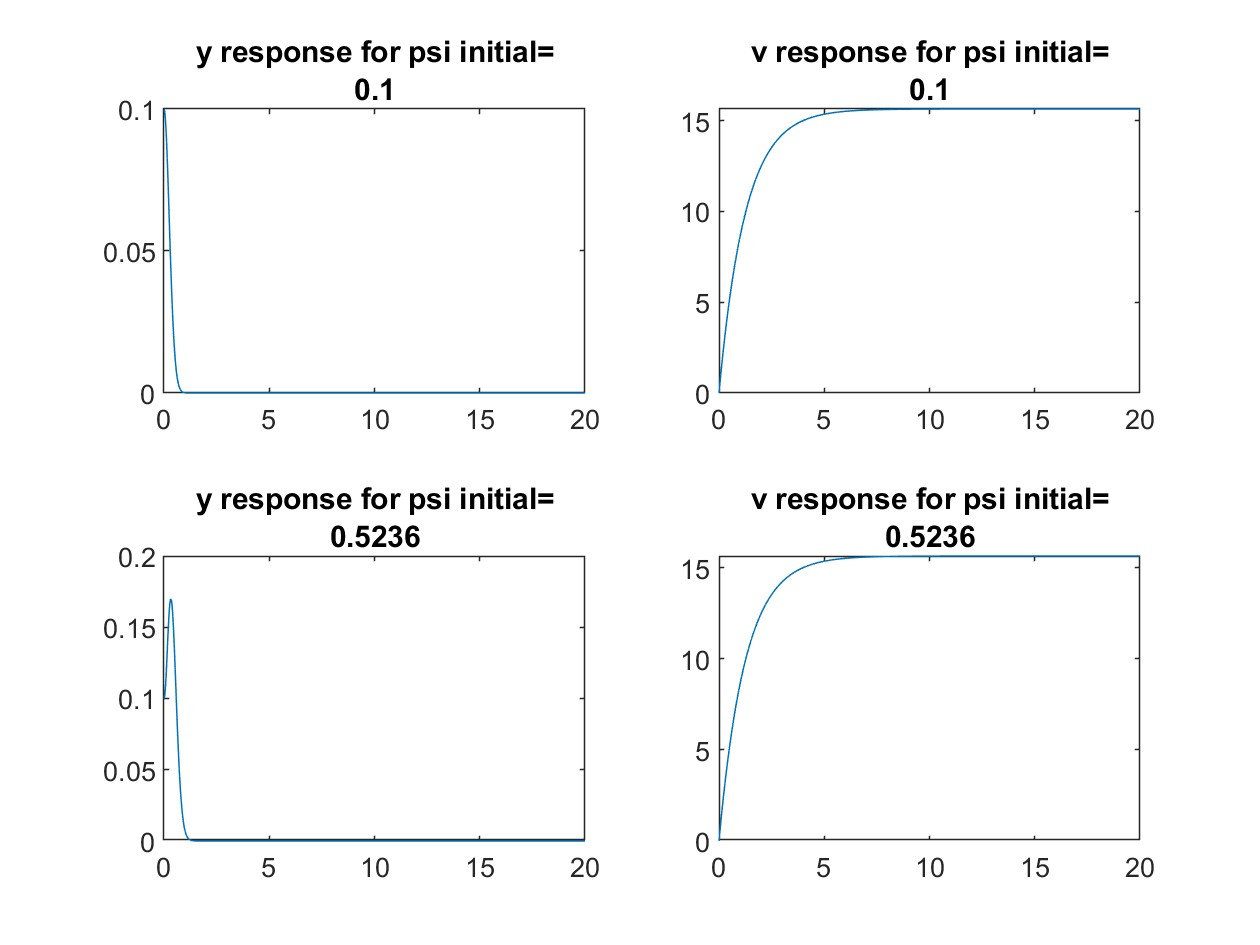
\includegraphics[scale=0.3]{Problem5Fig3.jpg}\\

Using the following code we can also plot out the velocity and y response for different $k_d$, to slow down the controller
regulating velocity we can increase $k_d$. We choose the slower velocity controller to have a $k_d=0.5$
\begin{verbatim}
v_target=15.6464;
y_target=0;
l_r=1.7;

k_p_v=1;
k_i_v=k_p_v^2/4;
k_d_v=0;
k_p_y=4/l_r;
t_final=20;
max_step_size=0.0001;

y_initial=0.1;
psi_initial=0.1;
v_initial=0;

a=sim("Problem5.slx");
t=a.tout;
y=a.yout.getElement("y").Values.Data;
v=a.yout.getElement("v").Values.Data;

subplot(2,2,1); 
plot(t,y)
title(["y response for velocity controller k_d=",num2str(k_d_v)])

subplot(2,2,2); 
plot(t,v)
title(["v response for velocity controller k_d=",num2str(k_d_v)])

k_d_v=0.5;
a=sim("Problem5.slx");
t=a.tout;
y=a.yout.getElement("y").Values.Data;
v=a.yout.getElement("v").Values.Data;

subplot(2,2,3); 
plot(t,y)
title(["y response for velocity controller k_d=",num2str(k_d_v)])

subplot(2,2,4); 
plot(t,v)
title(["v response for velocity controller k_d=",num2str(k_d_v)])
\end{verbatim}
With this code we get the following graph.\\
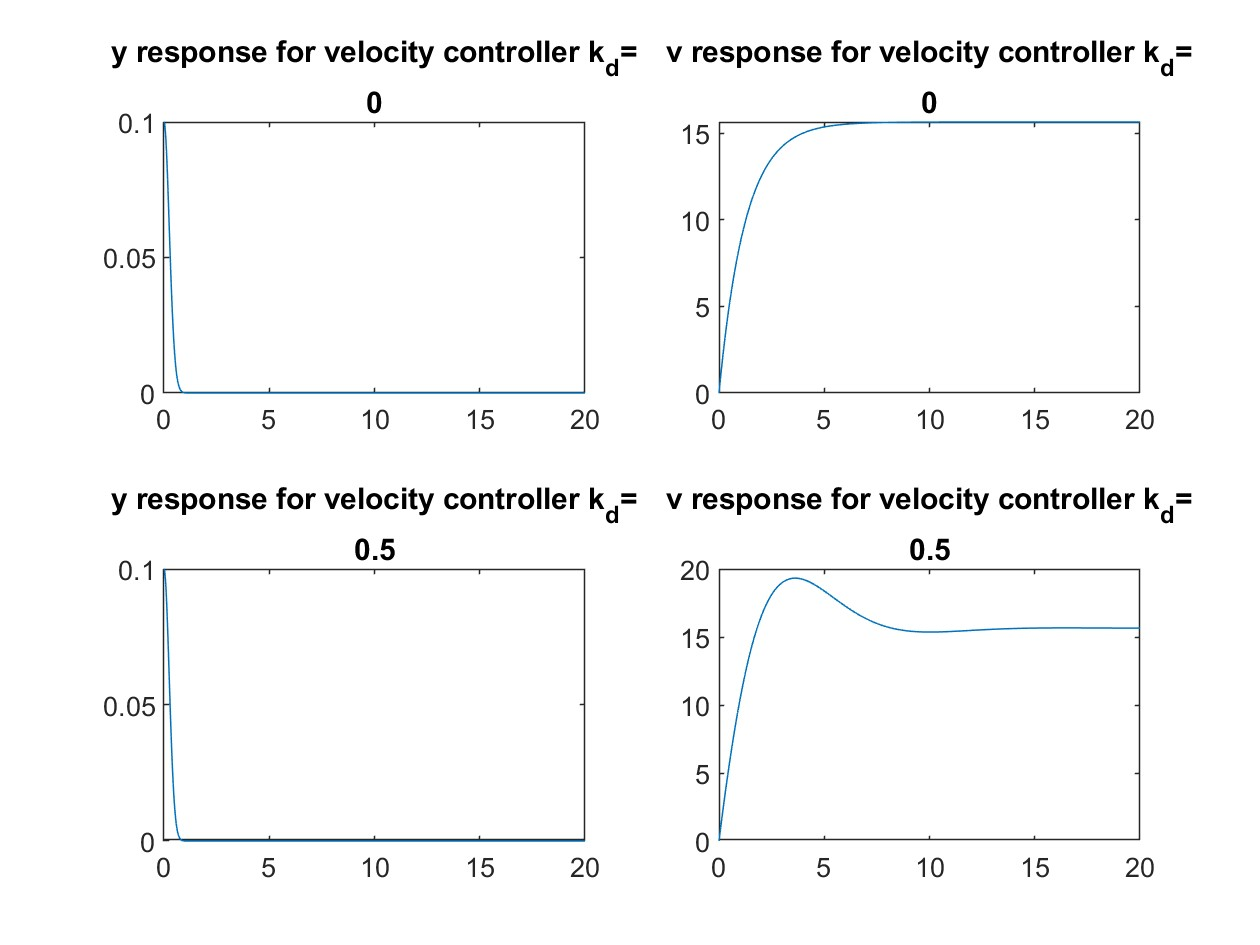
\includegraphics[scale=0.3]{Problem5Fig4.jpg}\\
As we can see, making the velocity controller slower does not seem to affect the y response, but as expected slows down the velocity response
and makes it underdamped.
\section*{Problem 6}
\end{document}